\section{Related Work and Conclusions}
\label{sec:rel-concl}

In the preliminary conducted experiments traces have been generated by a simple script and not through Java code instrumentation.
A simple solution to analyze real Java code is exploiting the the Java Logging API offered by module \lstinline{java.logging}.

Other more sophisticated tools have been proposed in literature. %The need to understand the behaviour of a Java piece of code is as old as Java itself. 

Early attempts to visualize Java programs date back to the end of the millennium. They were initially motivated by teaching reasons \cite{dershem1999java}, and became soon a fundamental engineering step for developing correct and safe Java applications \cite{DBLP:conf/wcre/Systa00,DBLP:conf/dagstuhl/PauwJMSVY01}. The Java visualization research strand is still active \cite{DBLP:journals/spe/JayaramanJL17,DBLP:journals/spe/PJJS21} but since -- in order to visualize a program behavior -- it is necessary to trace it \cite{DBLP:conf/dagstuhl/Mehner01}, most efforts are currently oriented towards the more general problem of Java tracing.
% and, being a requirement for tracing, of Java instrumentation. 

Different approaches to tracing exist, mainly depending on which part of the Java architecture, the bytecode, the source code, the JVM, is modified or instrumented to make the tracing possible.

In a work dating back 2001 \cite{DBLP:journals/fgcs/BechiniP01}, Bechini and Prete present a solution for tracing and replaying Java concurrent applications based on the automatic instrumentation of the original source code.

A less invasive approach is MuTT \cite{DBLP:conf/ACISicis/LiuX09} that works on top of JPDA (the Java Platform Debugger Architecture, available for old JDKs) and exploits JPDA features to collect the run-time information of multi-threaded Java programs without source code or JVM instrumentation.

More recently, JBInsTrace \cite{DBLP:journals/scp/CasertaZ14} computes complex dynamic metrics used to categorize programs according to dynamic metrics related to program size and structure, use of data structures, use of
polymorphism, memory footprint and concurrency. 
To this aim, JBInsTrace instruments and traces Java bytecode. It does not alter the JVM and does not statically modify class files. 
%Via tracing, static information about source code is produced, as well as a  fine grained trace of Java software execution, that allow detailed analysis of the runtime. 

When tracing takes place while the program is running, the effect of tracing is indeed a runtime monitoring of the program's behavior or, using the terminology adopted in this paper, its runtime verification.

Indeed, runtime verification of Java programs started to be addressed in 2001, when the Java PathExplorer was developed \cite{havelund2001java}. Java PathExplorer tested the execution traces of the Java program against high level specifications expressed as temporal logic formulae. An initial prototype of the tool was applied to the executive module of the planetary Rover K9, developed at NASA Ames. 

JASSDA \cite{BrorkensM02} was developed one year after Java PathExplorer. It is a RV framework for Java programs
based on CSP-like specifications and implemented in Java. JASSDA is very simple and does not support concatenation; parametricity
is obtained through slicing. 

PQL \cite{MartinLL05}  is an expressive language supporting RV of open-source Java
applications that allows specifications of properties covering the closure of context-free languages combined with intersection;
however, it does not support shuffle, and parametricity.  Its implementation is based on Java, Python and DataLog. 


LARVA \cite{ColomboPS09} is a RV tool expressly designed for checking real-time properties of Java programs.
Properties are specified in DATEs \cite{DATEs}
based on an extension of timed automata; in particular, it supports
symbolic states to guard transitions, replication of automata, and 
CCS-like communication between automata. LARVA is implemented in Java and code instrumentation is based on AspectJ.

SAGA  \cite{BoerGouw14} is another framework for RV of Java programs
based on attribute grammars. With attribute grammars it is possible to support parametricity and to mix specifications
with code instrumentation by exploring the full computational power of Java. Its implementation exploits Java, ANTLR and Rascal.

Differently to the other tools, \rml allows generic specifications fully independent from Java.
The specification provided in \Cref{sec:spec} can be reused for other Java-like languages, except for some renaming and adjustment
in the definition of event types, needed because of the different method signatures used in the libraries.

For what concerns future work, once traces can be generated from real Java programs with a specific instrumentation tool,
two challenges should be investigated:
\begin{itemize}
\item scalability of the approach: benchmarks with traces generated from real programs have to be considered, to assess whether
  the approach is scalable to verify real applications.
\item usefulness of the approach: experiments with Java programs extensively using hash tables should be conducted to understand
  how many true and false positives can be detected.
\end{itemize}

%% Table \ref{comparison} provides a summary of the comparison of RML with some of the most widely used tools for RV of Java programs, thas shows that 
%% RML is SUS-agnostic verification with a strong separation between instrumentation and specification of the properties to be verified. It supports parametricity, generics, and it allows to express non context-free properties. 

%% \begin{table*}
%%     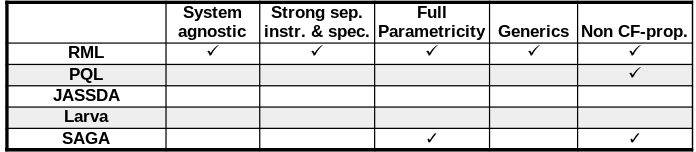
\includegraphics[width=0.6\textwidth,keepaspectratio=true]{tabella-viv3.jpg}[htb!]
%% \caption{Tools for RV of Java programs and their comparison with RML.}
%% \label{comparison}
%% \end{table*}
